\chapter[Big Data Analytics Platform]{Concept and Implementation of Big Data Analytics Platform}
\label{chapter:platform}
We have referred to big data platform concept and implementation on many occasions in previous chapters. In chapter \ref{chapter:background} we have discussed the basic concepts of big data with various technological advancements and solutions available for handling big data. In chapter \ref{chapter:method} we mentioned the functional components and their implementation during different stages, cycles and iterations. In this chapter we shall first explain the concept and a sample application framework for a big data platform based on available open source components. Then we shall present the part of this concept that we have implemented for handling the energy and social media data for our energy efficiency use cases listed in section \ref{use_cases} of previous chapter. 

Before we move to our conceptual model of the big data platform it is important that we mention basic challenges that drive the design of a big data solution and briefly explain a typical big data analytics process.

\section{Big data challenges}
As discussed in section \ref{bigdata_intro} of chapter \ref{chapter:background} there are five main challenges that influence the solution design criteria for big data analytic systems. These challenges are generally termed as 5V s of big data.
\begin{enumerate}
\item \textbf{Volume} refers to the size of the data. Volume is the most commonly associated feature with the big data. The big data analytics platform in our scope of work is based on Hadoop File Systsem (HDFS) which is a highly scalable system. It has been tested with upto 4000 scaled out serving nodes capable of handling upto 10 Petabytes (PB) of data.
\item \textbf{Velocity} refers to the data procesing speed.Velocity is crucial for the business use cases that need to process huge volumes of data in real time to produce insights for decision making. Our model is designed for batch processing, however we have integrated additional components that can process the data with near to real time capability.
\item \textbf{Variety} refers to structure of the data. Traditionally the relational data base system can store data with fixed schema. The fixed schemas mean that the stored data must have a definitive structure. Such databases are designed on basis of these data structures. In context to big data sometimes it is hard to perceive the structure of data so the storage systems needs to be designed for data in any structural format i.e. structured, unstructured or semi-structured formats. In our conceptual model we have added various components that can handle all formats of the data. However, In our implementation we shall be processing the data that had known fixed schema. 
\item \textbf{Veracity} refers to the complexity due to noises and inconsistencies of the data. In real life scenarios for big data it is very rare to find data in absolute consistent. Most of the time some values will be missing or the data will be in wrong format or there will pollutions in data. For good analysis we need to take care of such inconsistency and errors in data. Our conceptual model is capable of handling inconsistencies and in our implementation we had catered for some inconsistencies that we shall discuss in next chapter \ref{chapter:Analysis}. 
\item \textbf{Valuation} refers to the benefits of processing big data against the efforts required. It is an emerging feature for big data analysis design. Just like the other IT systems, organizations tends to decide about big data investments by looking at the business cases. In our concept we shall be discussing a model based on open source components. So there should be no cost of acquiring software. There is no specialized hardware requirements for implementing our model and any commercially available hardware with moderate specifications can be used to deploy this software. Hardware maintenance is required for running the service based on our model. However their are cloud alternatives that can be use within our model with some costs. However we shall not be discussing such alternatives in scope of this document or our research.    
\end{enumerate} 
\section{Data Analysis work-flow} \label{workflow}
 The data analysis process involves collection of data from multiple heterogeneous sources including both social media data, consumer data, sensors data, and already data from data servers or databases etc. The collected data in its original form can be ingested directly into Hadoop file system (HDFS). If required some filters can also be applied while collecting the data for efficient use of storage space. Collected data can be structured, semi structured or unstructured and some pre processing can be done to format it i.e. form a schema or structure that can be stored and accessed for data mining in database(s). A data mining engine with flexibility to plug and use various quantitative and qualitative research tools can then be used to analyse the data as per use case requirements. Data mining engine requires a feedback loop to pre-processing unit to adapt to the requirements of the use cases. Another feedback channel for processed data storage can be provided for direct data manipulations. Results of the data mining can be stored in the database. A RESTful API or data driver can be used to extract data from database for visualization frontends. Figure~\ref{fig:process} shows the high level process flow.
 \begin{figure}[!h]
   \begin{center}
     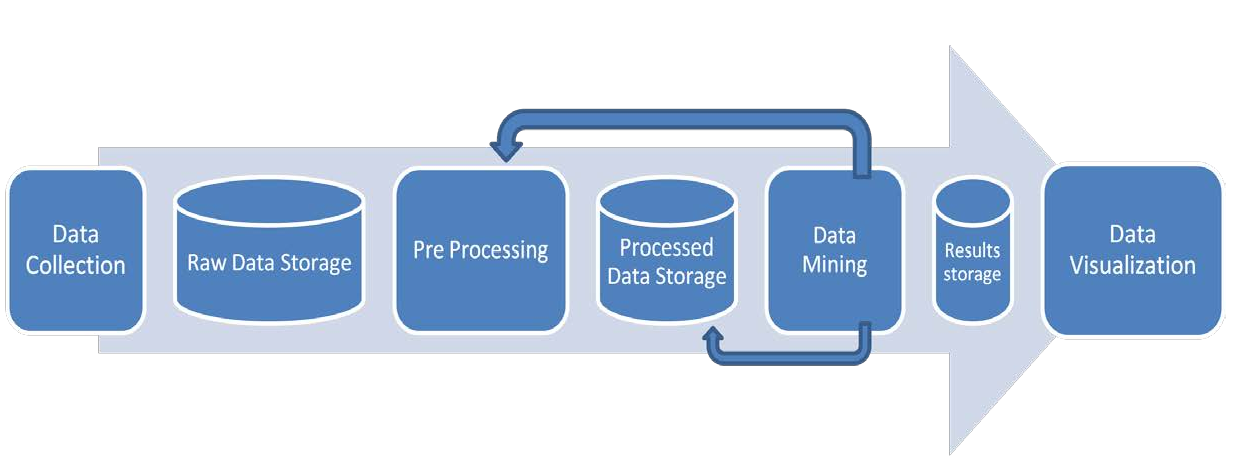
\includegraphics[width=\textwidth]{images/process.pdf}
     \caption{High level data processing flow.}
     \label{fig:process}
   \end{center}
 \end{figure} 
 \section{Platform concept}
 This section presents an end to end big data analytics platform aligned with the data processing flow described in previous section. The proposed platform is based on software components that are available open source free of cost. However use of each software components is subjected to its respective license under a specific open source licensing scheme. There are closed source and paid cloud services components available that can be used as efficient alternatives for parts of this model. However this paper does not contain information about these alternatives. Figure ~\ref{fig:cplatform} illustrate the proposed concept
 \begin{figure}[!h]
    \begin{center}
      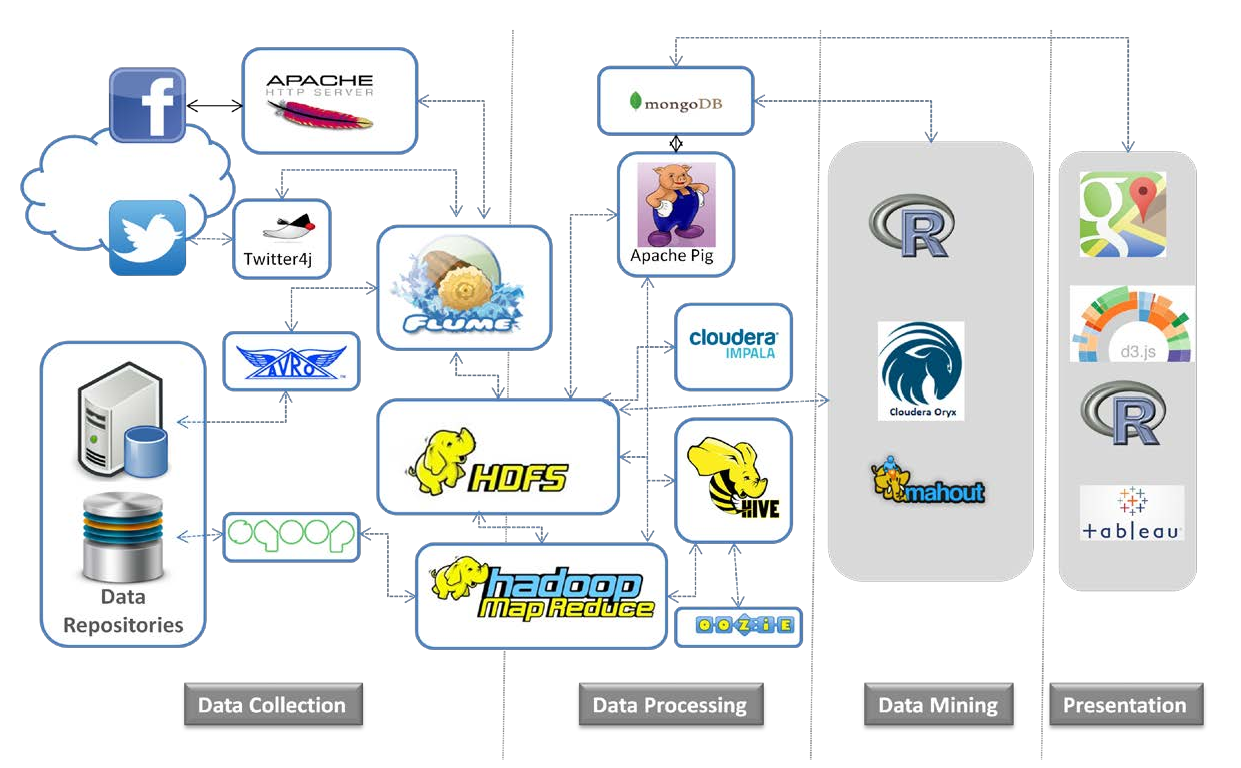
\includegraphics[width=\textwidth]{images/cplatform.pdf}
      \caption{Conceptual model of big data analytics .}
      \label{fig:cplatform}
    \end{center}
  \end{figure} 
\subsection{Data Core}
Before we go into details of each and every process step and respective components, it is beneficial to discuss the data core of the platform that is based on Apache Hadoop MapReduce and the Hadoop file system (HDFS).These two components are also shared between data collection and data processing steps.  Apache Hadoop is a framework that allows the distributed processing of large data sets across clusters of computers and HDFS is a distributed file system that provides high throughput access to application data\cite{apachehadoop} thus providing a highly efficient and scalable solution for handling big data. We have described Hadoop and MapReduce in section \ref{mapr}.
\subsection{Data Collection}
The proposed platform is capable of collecting and aggregating data from multiple data streams i.e social media data, consumer data, or server log files etc. The data can be live streaming data or data residing in server file systems or databases. Data can be collected as it is so there are no dependencies on format or structure of the data. Some filtering can also be applied while collecting data e.g. collecting only the geo tagged tweets or collecting logs with error notifications only. Following two components are recommended for data collection
\subsubsection{Apache Flume}
Apache Flume is a distributed service for efficiently collecting, aggregating and moving large amount of data \cite{flume}. Multiple flume agents can be configured to collect data from heterogeneous sources, channel the data to configurable destinations and store on desired locations. In the proposed model Apache flume is using Twitter4j library to stream data from Twitter, Apache HTTP REST API for collecting Facebook data and Apache Avro\cite{avro} data serialization system to collect log data from file systems of remote servers. Flume is then ingesting data directly into hadoop file system (HDFS). Flume can also read from databases and it is particularly useful while reading from document stores (NoSQL databases). However for reading from relational databases Apache foundation has another useful tool called Sqoop.
\subsubsection{Apache Sqoop}
Apache Sqoop \cite{sqoop} is designed for efficiently transferring bulk data between relational databases and Hadoop. So in most of the consumer data cases Sqoop can be used to collect data and feed it into HDFS through running multiple parallel Hadoop MapReduce jobs.
\subsection{Data Pre-processing}
Once the data is available in HDFS then it can be normalized to definitive structured forms e.g. schema. Furthermore, certain filtering can be applied for example in case of tweets, tweet text can be separated from other information for qualitative analysis and then natural language processing techniques can be applied to get it ready for further text mining. Usually pre-processing also helps in filtering out the unwanted information and make data lighter for mining process. In the proposed model Apache Pig and Hive are used to pre-process the data. Apache pig and hive both use Hadoop Mapreduce as parallel batch processing. For sake of fast pre-processing Cloudera Impala is also also added to the model.
\subsubsection{Apache Hive}
Apache Hive \cite{hive} is data ware house software that provides a way of providing schema to the stored data with SQL based query language to extract, transform and load data (ETL). Apache hive is further supported by another Apache Hadoop ecosystem tool called Oozie. Ooozie is acting as a workflow scheduler for Hadoop i.e. while loading the data into Hive it can create partition for tables arrange the data for optimized querying.
\subsubsection{Apache Pig}
Apache Pig \cite{pig}  provides a high level scripting language to analyze the data stored in HDFS using MapReduce. 
\subsubsection{Cloudera Impala}
In section \ref{mpp} we have already introduced Cloudera Impala as a massively parallel processing database engine. We also  explained the concept of massively parallel processing databases. In this section we shall emphasize on how Cloudera Impala fits into Hadoop ecosystem.
 
Cloudera Impala uses HDFS as its main data source. It can read data directly from a HDFS directories. The HDFS directory path can be configured before each run. Data can be read from a single or multiple files stored within the configured directory. A schema needs to be created inside Cloudera Impala. Based on schema it can project the data in HDFS directory files as a table. The data can then be queried using a subset of SQL (structured query language). Cloudera Impala provides much faster processing than Hive and Pig that uses parallel batch processing. However Cloudera Impala currently supports limited data structures. For handling some complex data formats e.g. Avro serialized JSON format data. For such cases it can be configured to work together with Hive and Hbase etc.\cite{cimpala} 

\subsubsection{Databases}
For storing the pre-processed data various choices of available open source databases can be applied in this platform. While document stores like MongoDB seems a natural choice because of the flexibilities to handle any structure data and easy maintainability but the relational databases can still be integrated and used within this platform. The availability of tools like Cloudera Impala can fit very well with SQL based databases like mysql to build online query engines. Apache Hive in this model is also acting as a projection on top of mysql.

\subsection{Data Mining}
The real value of any analytics platform lies in its ability to make sense of the data. Data collection and data pre-processing modules of the platform can bring and normalize data from multiple streams to be further analyzed by the data mining modules in the platform. There are various open source data mining and statistical analysis tools available online with power of most advanced machine learning, text mining and statistical modelling algorithms built in them.  The proposed platform can provide a plug n play environment for most of these tools to be applied on use case requirements. Some example of these tools as presented in figure 2 i.e. Apache Mahout, R Project, and Cloudera Oryx. 

R does not provide scalability or parallelism without special configurations. It process data in memory so it requires large RAM (Random Access Memory) for large data sets.The real power of R is in availability of large number of statistical and advance analytics algorithms. With proper data pre-processing using big data tools like Apache hive, pig and Cloudera Impala the amount of data processing can be reduced for R without loosing key insights.

 Apache Mahout and Cloudera Oryx can fit well with Hadoop ecosystem tools to provide scalability and parallelism for applying data mining and machine learning on big data. Cloudera Oryx is designed particularly for velocity. However it is still in development phase and has support for less number of data mining and machine learning algorithms. It is expected that it will take over Mahout completely if it can match the Mahout's algorithm library.  
\subsection{Presentation}  
For visualizations of the results, this model presents some tools to build interactive dashboards. These dashboards should be able to zoom in and out of data. They should provide flexible way of managing visualizations based on use cases. Also they can be integrated into user interfaces of web based or mobile applications. The suggested components are Tabelau Public, d3.js, google maps and R project.

Tableau public provides the easiest solution to visualize data through static and interactive graphs. Tabelau public is a free service. The paid version of Tableau can give additional tools like connecting directly to data bases and Hadoop ecosystem tools like Apache Hive. Tableau software are based on VizQL (Visual Query Language) paradigm \cite{hanrahan2006vizql}. Once connected to the data source VizQL  provides a very flexible way of interacting with graphs. The idea is to focus on the insights that are required rather than spending more efforts on programming the queries to generate those insights. Tableau automatically generates the queries and visualize the results.

D3.JS provides a comprehensive library in Java Script for making customized information graphics. It is very flexible and powerful. However it need programming skills in Java scripts and a reasonable effort is required to prepare or change the graph formats. 

Google maps is a powerful tool for geo-spatial info graphics. In many big data use cases geo spatial mapping provides a smart way of presenting information.

R - project also have additional packages and libraries like ``ggplot'' to visualize the results after applying statistical analysis and data analytics. Like D3.JS R infographics also need programming to visualize the results.

\section{Implementation}  
In this section we shall be discussing our implementation for analysing the energy consumption data for our energy efficiency use cases and collecting social media data for supporting CIVIS project. The implement model is the subset of the conceptual model presented in previous section with at least one additional component that we shall discuss later in this section. Figure~\ref{fig:iplatform} shows the implemented model. The details of configurations are available in Appendix \ref{chapter:appendixb}.  
\begin{figure}[!ht]
    \begin{center}
      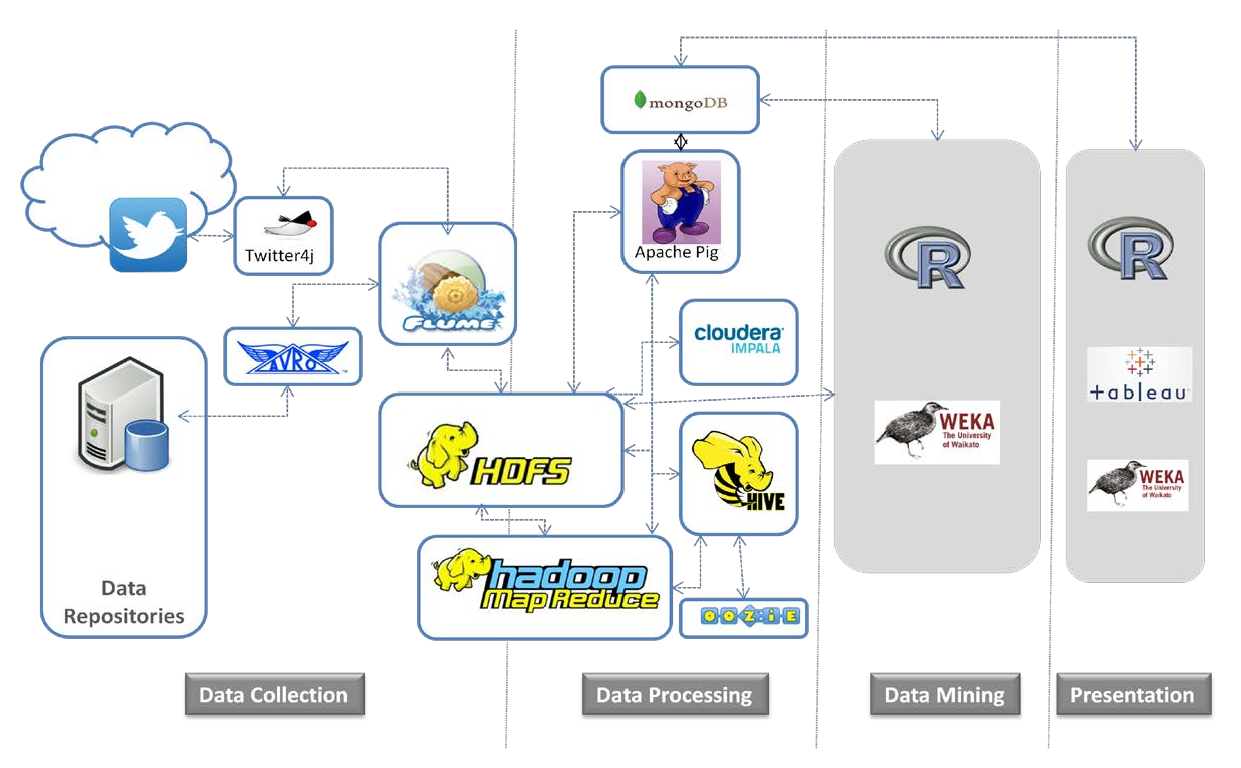
\includegraphics[width=\textwidth]{images/iplatform.pdf}
      \caption{Implemented big data analytcis platform .}
      \label{fig:iplatform}
    \end{center}
  \end{figure} 
\subsection{Implementation Environment}
Cloudera distribution including Apache Hadoop (CDH) version 4.7 was used for implementation of our big data analytics platform. Following is the list of the components used with their respective version numbers.  
\begin{longtable}{@{}p{0.5\textwidth}p{0.5\textwidth}@{}}
Apache Flume & flume-ng-1.4.0+97 \\
Apache Hadoop (MapReduce\(+\)HDFS) & hadoop-2.0.0+1603 \\ 
Apache Hive & hive-0.10.0+258 \\ 
Apache Oozie  & oozie-3.3.2+102 \\
Apache Pig & pig-0.11.0+43 \\ 
Cloudera Impala & Impala 1.3.1 
\end{longtable}
Cloudera CDH 4.7 was used in form of a pre-configured quick start virtual machine (VM) capable of running on top of any known operating system e.g. Microsoft Windows xp/7/8 , Linux RHEL/Centos, and Ubuntu etc. Cloudera CDH 4.7 quick start VM itself was running on Centos 6.2 operating system. Following Hardware resources were allocated to run the VM for our analysis.
\begin{itemize}
\item 3 x 1.8GHz intel i7 4500 CPU
\item 4GB RAM 
\item 64 GB VMDK storage
\end{itemize}
During testing phase we have also test multi node cloudera CDH 4.7 configuration on cloud. However there was cost associated to running the set up on cloud and the requirement of our use cases were also fulfilled by single node quick virtual machine. So we preferred not to run analysis using multi node cloud deployment.

In addition to pre-configured components in Cloudera CDH 4.7 we also added some additional components as part of our platform. Following is the list of those components with their respective versions.
\begin{longtable}{@{}p{0.5\textwidth}p{0.5\textwidth}@{}}
Apache Avro & v 1.7.6 \\
R & v 3.0.3 \\ 
Tableau & public , v 8.0 \\ 
Weka  & v 3.7 \\
Twitter4J & v 3.0.3 
\end{longtable}

For ease of use we had been using R, Weka and Tableau outside quick start VM environment. Typically we were using Windows 7 with similar dedicated hardware resources as for quick start VM. Tableau public is a web service running in public cloud.
\subsection{Implemented data processing work flows } 
As mentioned before, we utilized the implemented platform for two purposes.
\begin{itemize}
\item Analysing energy data for energy efficiency use cases.
\item Collection of social media data to support CIVIS project activities. 
\end{itemize}
In this section we shall explain the data processing work flows for both scenarios. These work flows are aligned with the process we explained in section \ref{workflow}. 
\subsubsection{Data processing for energy efficiency use cases}
For analysing the energy consumption data, we designed and implemented the platform to automatically collect data from VTT's data servers and ingest it into Hadoop Files System. For data collection we configured Apache flume to collect and aggregate the data. Apache Avro was configured within Apache Flume to serialize the data. Unfortunately due to some policy issues at VTT, we were not allowed to integrate our platform to there data servers. Instead data was provided to us through an FTP server. In later stages we were also given access to a web service from which we can download data in off-line mode. Here off-line mode means that data was not collected automatically and human intervention was required to collect the data.

The collected data was then ingested to HDFS manually. Once the data is available on HDFS then data pre-processing tools can access it. Selection of the preprocessing tool is based on use case requirements, format and volume of data. As discussed before, VTT provided us two types of data i.e. hourly electricity consumption data from smart metering devices and second set of NIALM device level data. For first data set of hourly electricity consumption data we used Apache Hive to pre-process the data. The decision was based on the fact that data had fixed schema and Hive has good support for such data types. Alternatively, Apache Pig and Cloudera Impala could have also been used but a choice was made on basis of preference. For performance test purposes we had used Cloudera Impala and Apache pig. We shall discuss details of that in next chapter. For data analysis purpose following schema was created in hive and data was loaded as per following schema.
\begin{lstlisting}
CREATE EXTERNAL TABLE hourly_data
(
   devid string,
   building string,
   meternumb int,
   type string,
   day string,
   hour int,
   consumption int

)
ROW FORMAT DELIMITED FIELDS TERMINATED BY ','
\end{lstlisting}

 After loading the data was processed to prepare inputs for data mining and advance analytics modules as per use case requirement e.g. for classification on basis of energy efficiency the input matrix for K-means algorithm was produced. For producing this input matrix ~1.2 Million records \((rows)\) were reduced to 343 rows. Making it very simple for R to apply K-means algorithm. Then from R we saved the results of classifications to comma separated file. This file was then read by Tableau Public. We then generated the visualizations for our analysis. Tableau can connect to data files in live mode so the updates in files can directly be imported and projected on created visualizations. However this was not required for our case.
 
 For the second data set of NIALM device data, volume of the data was too small. So we analysed it in R without pre-processing. We used both R and Weka to apply and evaluate different analytics techniques. Weka was used only in evaluation step as describe in section \ref{eval} as it provides a quick mechanism for analytics prototyping. It can not be used in tight integration within platform so our conceptual model does not include Weka as an option. For visualizations we used R plots and Weka graphs.
 
 \subsubsection{Social media data collection for supporting CIVIS project}
 To support CIVIS project activities we configured our platform to collect and store Twitter data using Twitter streaming API. The implementation procedure for achieving this case was based on a Cloudera Tutorial ``How-to Analyze Twitter Data with Apache Hadoop'' \cite{clouderatwitter}.
 We configured Apache Flume with Twitter4j Java library to  capture the twitter stream data. A twitter application was registered with our Twitter account to get the access to streaming API. The keyword filtering was applied using twitter4j to target the concerned tweets only. Tweets were then stored to HDFS by Apache Flume HDFS sink mechanism. Hive table was created with the a subset of twitter provided schema. This helped us in shedding the unwanted header data to reduce the storage size. Apache Ozie workflow was implemented to archive hive data in manageable format i.e. creation of twitter data partitions on basis of hourly data. This is a very helpful feature in reducing the query processing time. Within our scope we did not analyse the twitter data.    
